\documentclass[tikz,border=9pt]{standalone}
\usepackage{amsmath,amssymb}
\usetikzlibrary{arrows.meta,positioning,calc}
\begin{document}
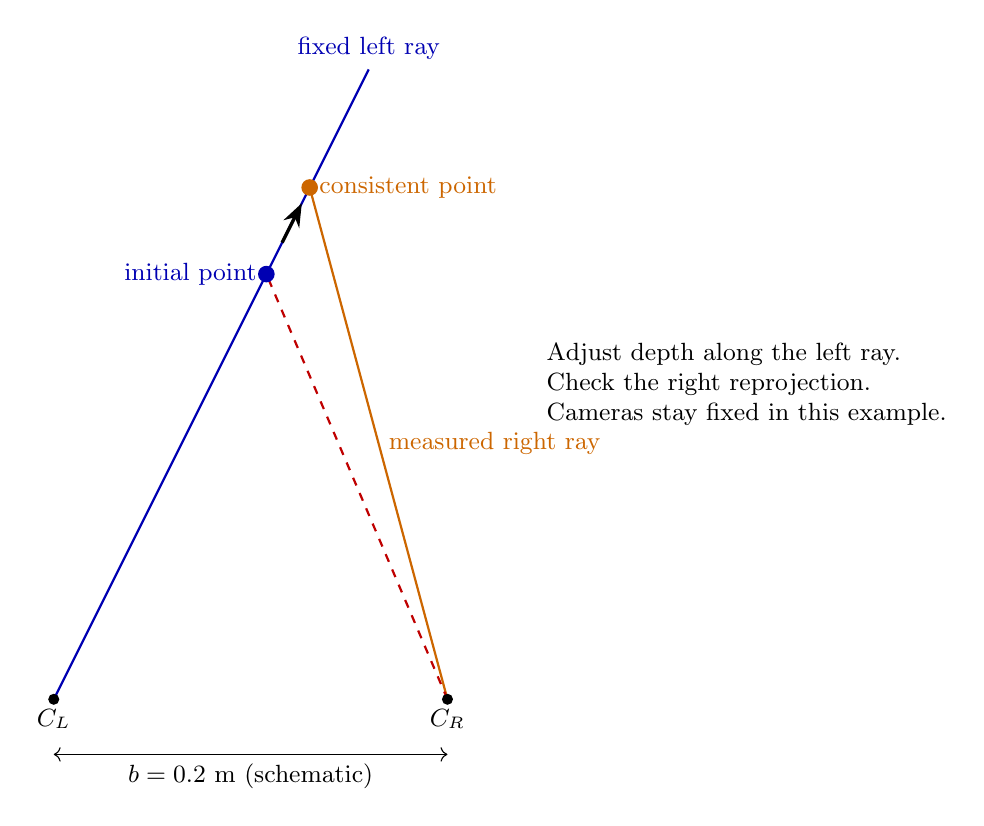
\begin{tikzpicture}[font=\small,arr/.style={-{Stealth},thick},box/.style={draw=blue!55!black,rounded corners,fill=blue!4,align=center,text width=2.9cm,minimum height=1.05cm}]

\coordinate (L) at (0,0);\coordinate (R) at (5,0);\coordinate (T) at (3.25,6.5);\coordinate (Q) at (2.7,5.4);
\draw[thick,blue!70!black] (L)--(4,8) node[above]{fixed left ray};
\draw[thick,orange!80!black] (R)--(T) node[midway,right]{measured right ray};
\draw[dashed,red!75!black,thick] (R)--(Q);
\fill (L) circle(2pt) node[below]{$C_L$};\fill (R) circle(2pt) node[below]{$C_R$};
\fill[blue!70!black] (Q) circle(3pt) node[left]{initial point};
\fill[orange!80!black] (T) circle(3pt) node[right]{consistent point};
\draw[arr,very thick] (2.9,5.8)--(3.15,6.3);
\node[align=left] at (8.8,4){Adjust depth along the left ray.\\Check the right reprojection.\\Cameras stay fixed in this example.};
\draw[<->] (0,-.7)--(5,-.7) node[midway,below]{$b=0.2$ m (schematic)};

\end{tikzpicture}
\end{document}
